\chapter{Related Work}

\section{Ad-hoc methods}
	Simple distortion methods are applied to the image privacy protection field such as pixelation and blurring. The pixelation method subsamples the image and the blurring method smoothes images with some filters like Gaussian filter or average filter ~\cite{Agrawal09,Boyle00}. Both by destorying the original image information, pixelation and blurring make a trade between privacy information and image quality. Although these two methods are widely used in practical situations like TV interviews, they suffer from the same risk proposed in ~\cite{Newton05} called parrot attack. General face recognition algorithms figure out the identity by computing the similarity between the target image and database images. Blur and pixelation destory the target image information so that the target image is not similar to any image in database. Parrot attack would preprocess all the database images with pixelation or blurring, then applies face recognition algorithms to pixelated or blurred images so that target images and database images are preprocessed with the similar procedures. 

	\par
	Two more de-identificaiton methods are introduced in ~\cite{Winkler14}: blanking and encryption. The intuitive blanking method in face de-identificaiton is to cut the face region off and replace the region with black color. It also could be extended to paint the region of interest, like face, with background images  ~\cite{inpaint09,Qureshi09}. Compared with other de-identification methods introduced before, encryption has the advantage in recovery ~\cite{Boult05}. With a proper key, the encrypted image is always available to be decrypted so that the image remains useful even if it is covered by a snowboard. These two methods cover image information including both identity and facial expressions. It is the balance between privacy and data utilization that should be the key point in face de-identification. Protecting the identity privacy while preserving facial expressions simultanously is the purpose of our research. 
	
	\par
	Dufaux ~\cite{dufaux08} introduced a privacy protection method using in video sequence by scrambling the locations of pixels in a rectangle range. By controling the range size, different degrees of fuzzy results could be produced. 

	The images comes from ~\cite{dufaux08}.
	% whether place four images here
	\begin{figure}[!htb]
		  \centering
		  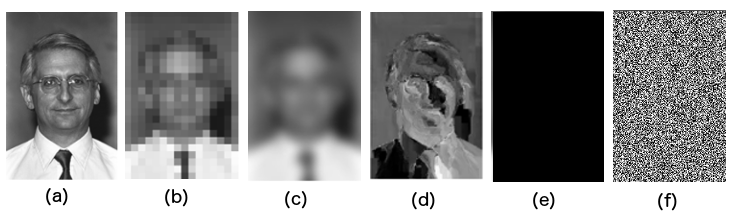
\includegraphics[width=0.9\textwidth]{figure/adhoc.png} 
		  \caption{(a) the origianl image; (b) Pixelation; (c) blurring; (d) scrambling; (e) blanking; (f) encryption}
		  \label{expression}
	\end{figure}


\section{K-anonymity based methods}

	General solutions model face shape and appearance separately. 